%\section{Introduction}

\section{Motivation of the research}

\subsection{Web applications and infrastructure}

Today, a great number of people in the world can not spend a day without using smartphones or personal computers(PCs) to retrieve information from the Internet for work or for daily life.
For example, people use these devices to look up web pages, emails, social media and sometimes to play games.
These services are often called web applications, where information is delivered using Hyper Text Transfer Protocols(HTTP) or Hypertext Transfer Protocol Secure (HTTPS) from servers at the other end of the Internet.
Web applications are provided by various organizations, including commercial companies, government, non-profitable organizations, schools, etc.
(The author calls them web application providers hereafter.)
A client program on PCs or smartphone sends out requests to servers and the servers respond with data that is requested, using HTTP or HTTPS. 

Servers for web applications are usually computers located in a data center.
%Servers also refer to the server programs that are runing on these computers. 
In the data center multiple servers cooperate to fulfill the need of the clients.
A group of these servers is often called a web application cluster or a web cluster.
Figure~\ref{fig:web_cluster} shows schematic diagram of an example of a web cluster.

\begin{figure}[h]
\begin{center}
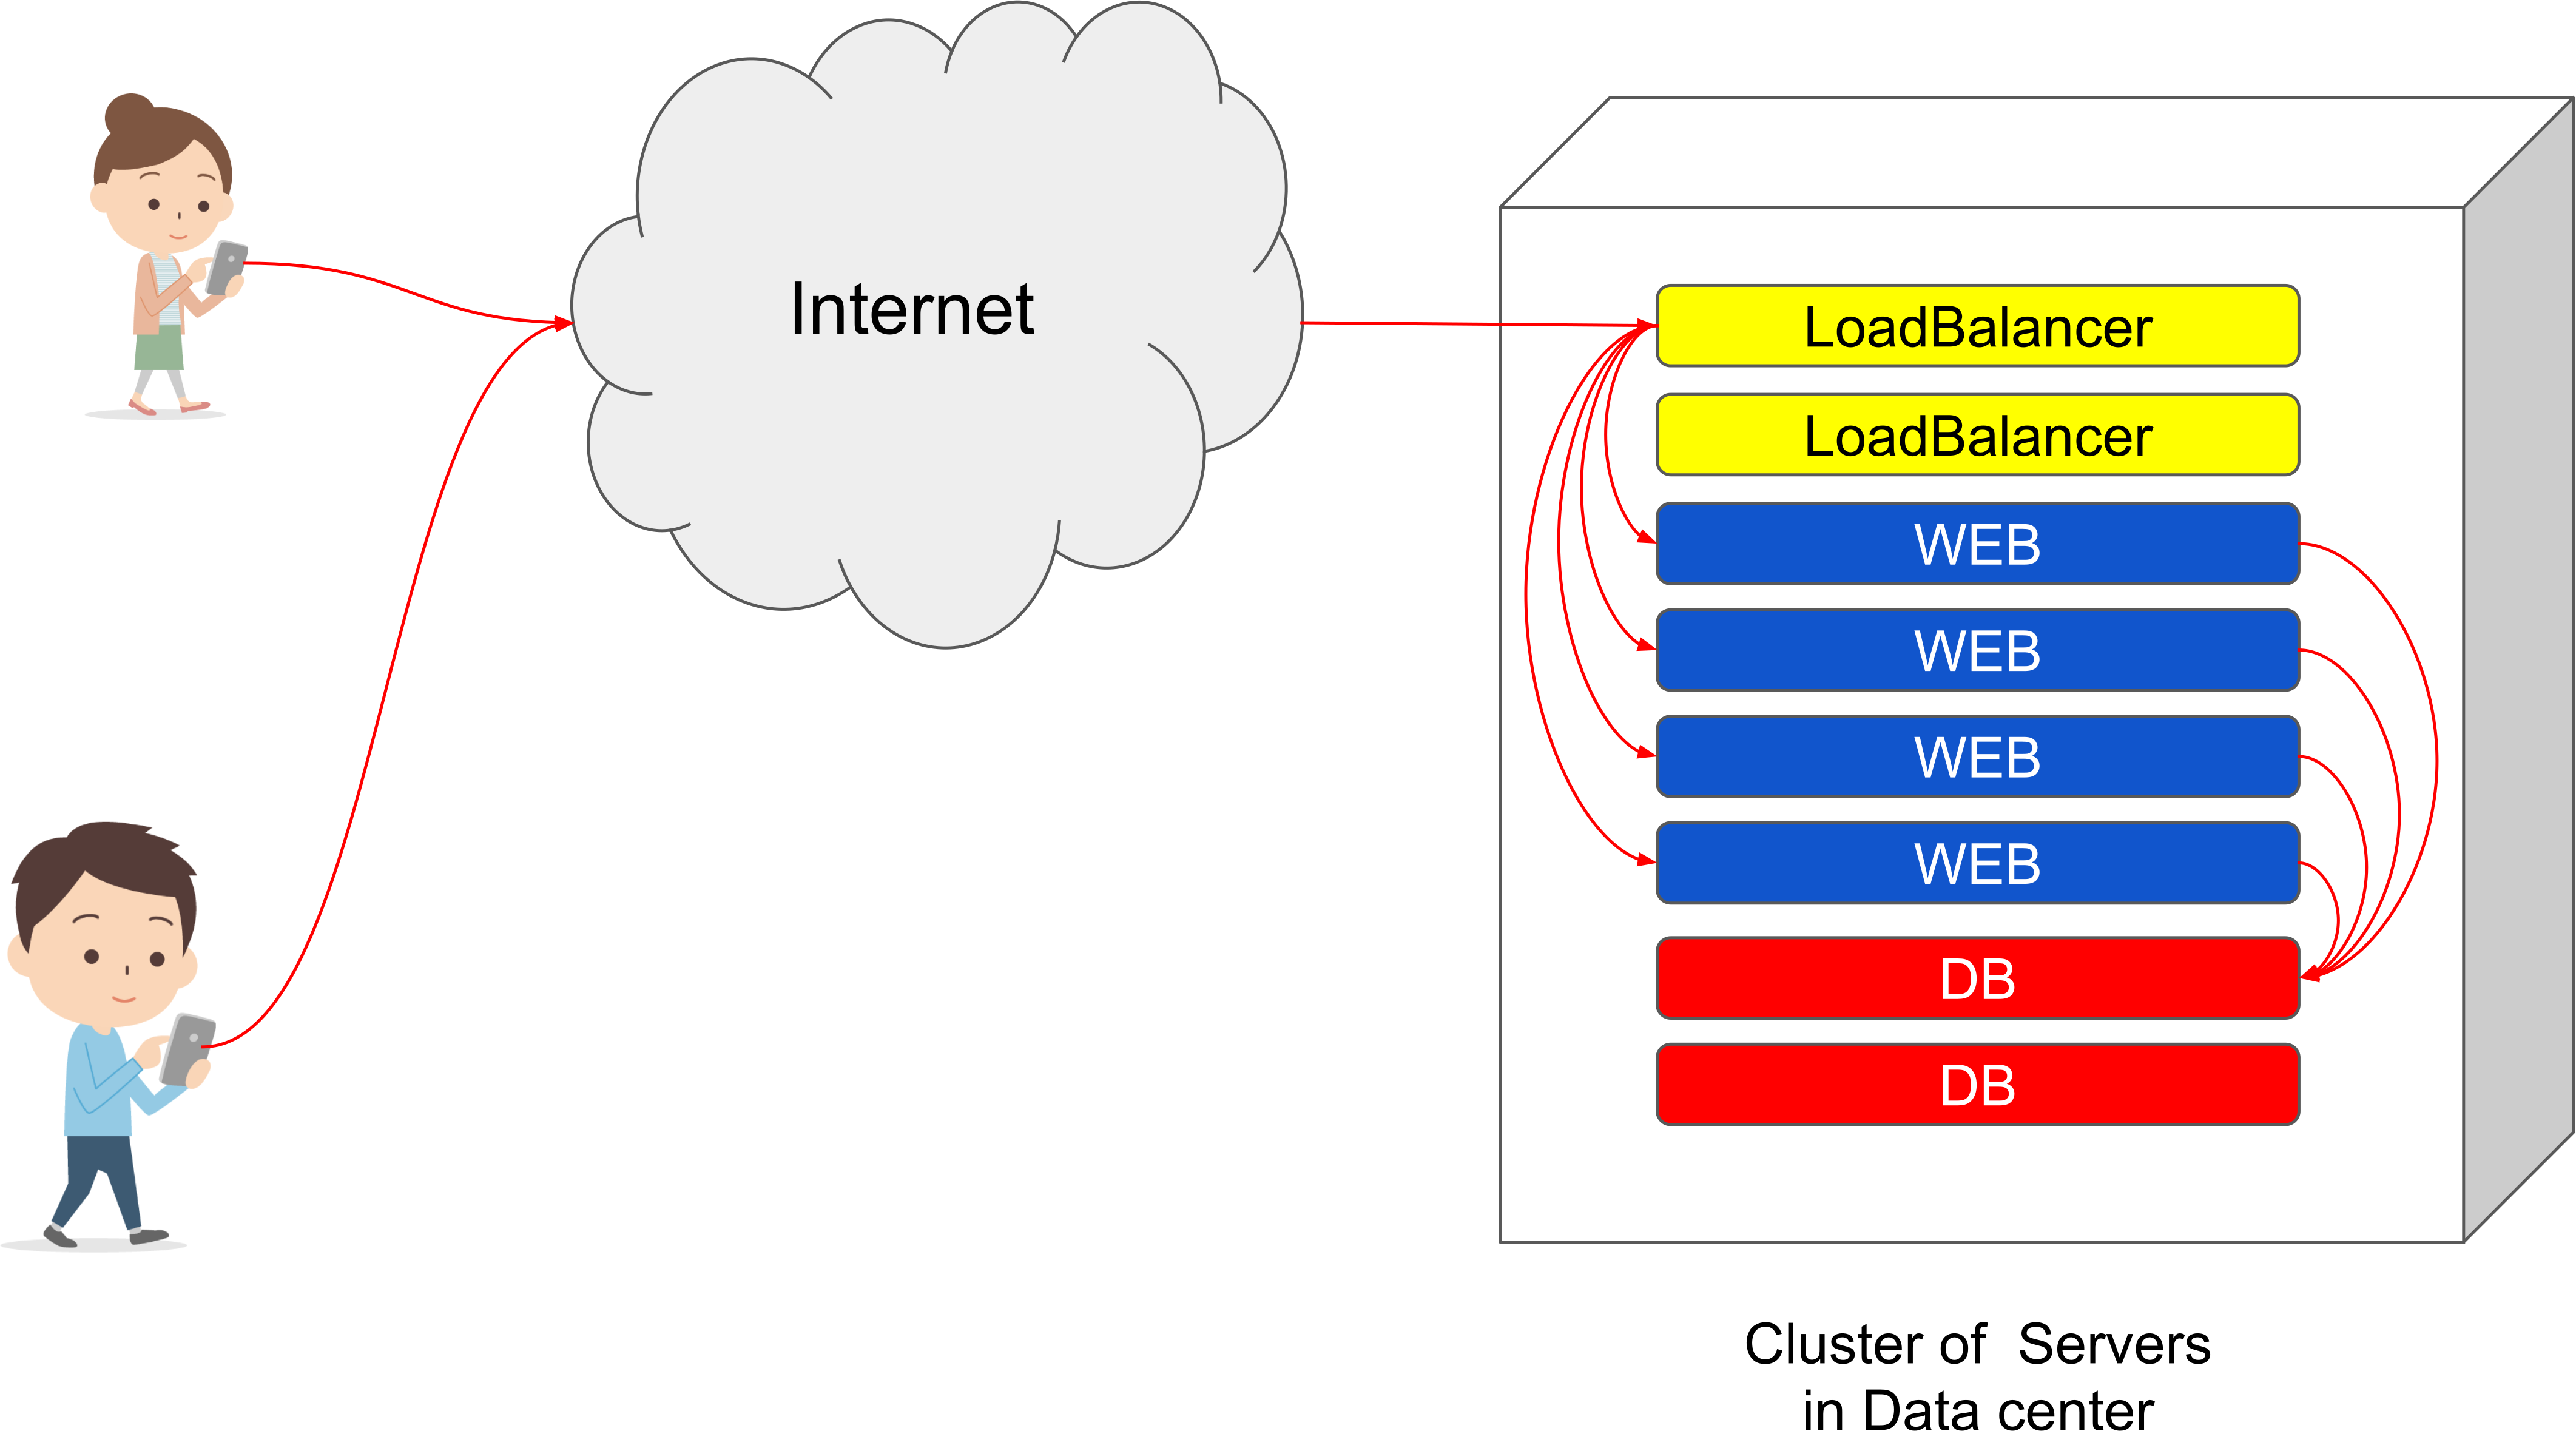
\includegraphics[width=0.8\columnwidth]{Figs/web_cluster.png}
\end{center}
\caption{
An example of web cluster.
}
\label{fig:web_cluster}
\end{figure}

In this example, there are two load balancers, four web servers and two Database(DB) servers that work together to respond to requests from clients.
The load balancers distribute requests from clients to multiple web servers. 
Then the web servers form the response using the data retrieved from the database servers, and send it back to the client.
Sometimes the web servers may store and update important data into the database servers.

\subsection{On-premise data center}

Web application providers often purchase these servers and locate them in server housing facilities called data centers.
In this type of infrastructure, the web application providers typically need to sign a contract with data center company for server housing racks, buy servers and install them in their rented racks by themselves.
Since the servers are located in the users own facilities or rented facilities, and the users are responsible for managing those servers, this type of infrastructure is often called on-premise infrastructure so as to contrast Cloud Computing infrastructure.
Preparing data centers, installing the servers and configuring software stacks for their services often require considerable amount of time, money and effort.
If web application providers want to expand their services to different countries or if they want to prepare for natural disasters by preparing an additional web cluster in a different data center, they most likely need about the same amount of time, money and effort required to build their original infrastructures.

\subsection{Cloud computing}

The emergence of Cloud Computing made many things easier for web application providers than before.
Cloud computing utilizes a virtual machine(VM) technology, e.g. KVM, Xen, and VMware.
Cloud computing service providers offer VMs to web application providers(users) with pay-per-use billing.

Figure~\ref{fig:physical_vm_container} (b) shows an example architecture of VM technology. 
VMs share a single physical server.
A full OS including Linux kernel is running on top of the virtual machine represented by the hypervisor.
Each VM behaves almost as same as a single physical server.
Since VMs are fractions of a single physical server, server resources are utilized with finer granularities.
Users can start their services with a cluster of VMs, which is smaller than a cluster of physical servers, and hence resulting in lower cost.
Cloud providers generally prepare physical servers and software stacks for VMs before renting it to users, and they also provide an easy to use web interfaces. 
As a result, users need only to click a few buttons on web browsers, before up-and-running VMs are available for them.
This easiness will bring agility to users when they launch their services.
And since computing resources are offered with per-second pay-per-use billing, users can quickly reduce the cost by stopping excessive VMs, when the demand for computing power decreases.
This was impossible when web application providers purchased physical servers and installed them in a conventional on-premise data center.
In short cloud computing brought the users agility, flexibility, and cost-effectiveness.

\begin{figure}[h]
\begin{center}
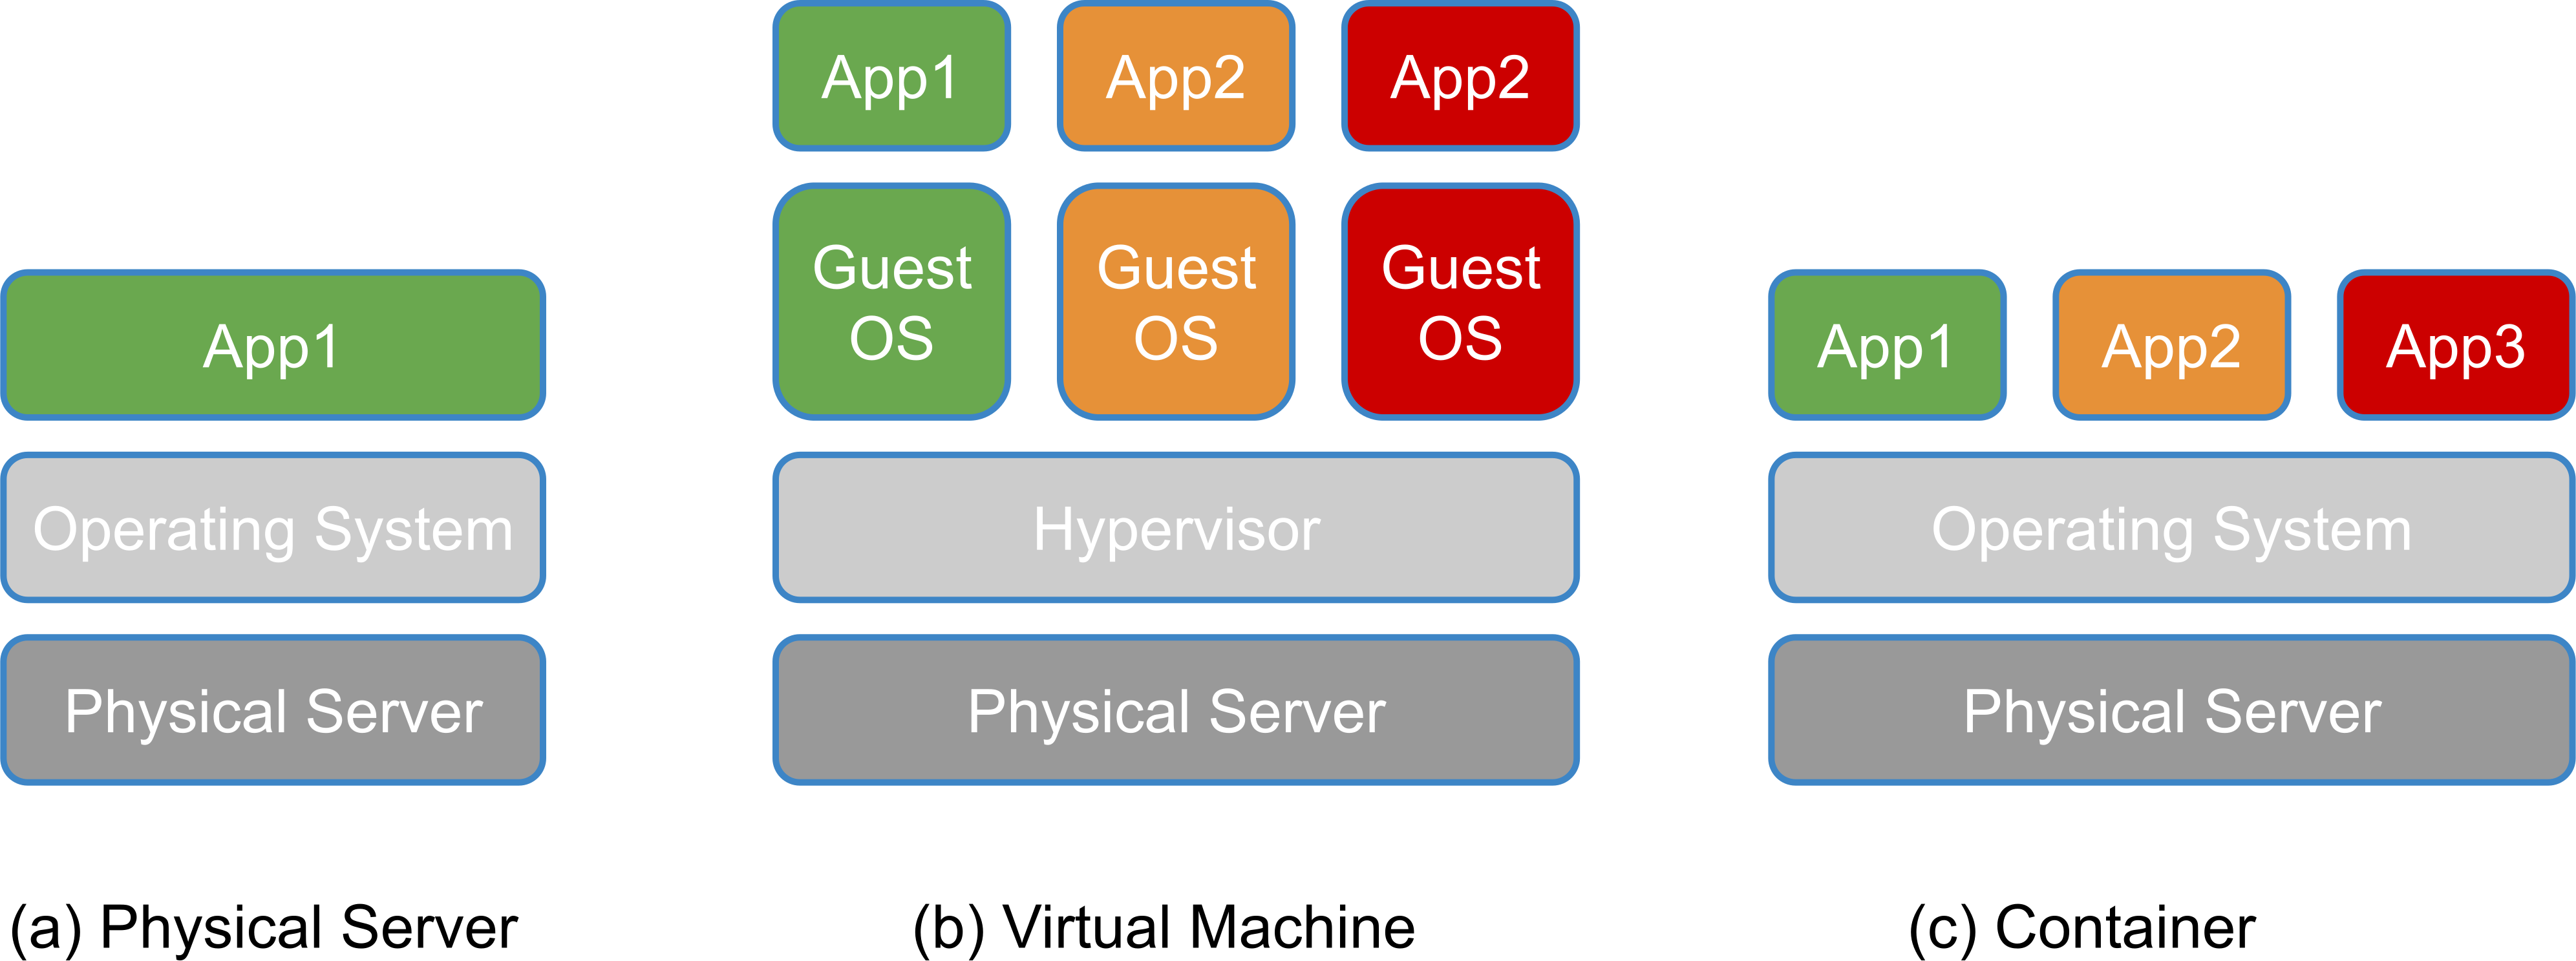
\includegraphics[width=0.8\columnwidth]{Figs/physical_vm_container.png}
\end{center}
\caption{
The difference in physical server usage between (a) Bare Metal servers, (b) Virtual Machine and (c) Container technology.
}

(a) Bare Metal servers is a word to describe conventional physical servers in contrast to Virtual Machines.
On top of a Bare Metal server, an operating system and application programs are running.
(b) Virtual Machine technology utilizes physical server hardware and a hypervisor.
The hypervisor provides generic representations of server hardware, which are called virtual machines.
A full operating system and applications are running on each of the virtual machines.
(c) Container technology separates applications by containing them to their respective namespaces.
Applications can not see each other's file systems, networks, users and process IDs unless they belong to the same namespace.
Since container technology merely relies on Linux kernel's namespace function and optionally cgroup, a containerized process does not have any additional overhead compared with a process running on a conventional physical server and operating system.
Container technology can be also utilized on top of virtual machines.

\label{fig:physical_vm_container}
\end{figure}

\subsection{Container technology}

More recently, Linux containers\cite{menage2007adding} have come to draw a significant amount of attention.
Figure~\ref{fig:physical_vm_container} (c) shows an example architecture of container technology. 
Container technology utilizes Linux kernel's namespace feature to separate process execution environments.  
Due to the widespread usage of Linux systems, Linux containers can run in most of the cloud infrastructures and on-premise data centers.

Every process is assigned to a certain namespace, and if two processes belong to different namespaces, they can not see each other's resources. 
Linux kernel implements filesystem namespace, PID namespace, network namespace, user namespace, IPC namespace, and hostname namespace. 
For example, each filesystem namespace can have its own root filesystem, and each network namespace has its own network devices and IP addresses.
Therefore, it is possible to configure processes as if they were running in different Linux systems by assigning them to different namespaces, although they share kernel and hardware.
Whilst VMs needed to run a full OS on top of a hypervisor and hence imposing extra overhead, a process in Linux containers is as light as a single process because it is merely a process that belongs to its own namespace.

Several management tools are available for Linux containers, including LXC\ref{}, systemd-nspawn\ref{}, lmctfy\ref{} and Docker\ref{}.
These tools take care of assigning an appropriate namespace to a process and make it look like running in its own virtual server.
For example, container tools restore a file system from an archive file every time a container is launched. 
Container tools also set up separate network interfaces with separate IP addresses in the container's namespace.

The fact that each container has its own file system that is restored from a single archive file means that a program binary and shared libraries are always exactly the same regardless of the base infrastructure.
Therefore a process in a container is expected to behave exactly the same manner, even if totally different data centers or cloud providers are used.
This was not easy when there was no container technology.
Because there are many flavors of Linux distributions, and even if the same distribution is used, there was always a chance that a slight difference in a program or library version could have broken the expected behavior.

A significant benefit of the Linux container technology is that it guarantees a process to behave always the same manner wherever the container is launched.






\subsection{Container Management System}

Thanks to benefits mentioned above, i.e., Linux containers are generally more lightweight, portable and reproducible than virtual machines(VMs), container technologies are very attractive for web applications. 
However in order to easily deploy web applications on top of a cluster of physical servers, container cluster management system or container orchestration tools are very important.

Orchestration tools do;
scheduling of containers


cloud providers are starting to offer services utilizing container technologies.
These service include tools that enhance the easiness of deploying a container management system  

For these reasons, Linux containers are attractive for web applications as well, and it is expected that web applications consisting of a cluster of containers can be run anywhere regardless of the difference in base infrastructures, i.e. cloud providers or data centers.


Ingress Routing Loadbalancing
Internal Routing Loadbalancing
Scheduling containers
Application definition

\begin{table}[H]
  \centering
  \begin{tabular}{|l|r|r|r|}
    \hline
    & \multicolumn{1}{c|}{Kuberenets} & \multicolumn{1}{c|}{Docker Swarm} & \multicolumn{1}{c|}{Mesos Marathon} \\ \hline
    Ingress loadbalancing & External & External & Static to Marathon LB  \\ \hline
    Internal loadbalancing & proxy setup iptables DNAT  & L4 routing mesh(ipvs) & Marathon LB(haproxy)  \\ \hline
    Container scheduling & Yes  & Yes & Yes  \\ \hline
    Application definition & Yaml & Yes & Yes  \\ \hline
  \end{tabular}
  \caption{Performance levels in 1Gbps and in 10Gbps.}
  \raggedright
  Throughput results of the load balancers at 40 nginx pods from the data for the Figures~\ref{fig:ipvs_l3dsr_1g.png} and \ref{fig:ipvs_l3dsr_10g} are shown.
%  \label{table:nat_tun_dnat_1g_10g}
\end{table}



Docaker Swarm, Kubernetes, Marathon
Container orchestrator.

Container management system schedule containers

Another aspect of the container management system is interesting. 
It can be viewed as the Operating System for a cluster of servers, where it not only provides scheduling of processes but also route the traffic to the right processes.
In this way, a cluster of computers can be used to provide web services with the ease of using a single computer.



migrated easily for a variety of purposes.
For example disaster recovery, cost performance optimizations, meeting legal compliance and shortening the geographical distance to customers are the main concerns for web application providers in e-commerce, gaming, Financial technology(Fintech) and Internet of Things(IoT) field.

The purpose of this research is to enable web application providers to easily deploy their services across the world seamlessly, regardless of cloud providers or data centers they use, by better-utilizing container cluster technology. 
Also, the author aims to realize the future where users can choose whatever infrastructure they like without sacrificing advanced features that are provided only by limited cloud providers.


\subsection{Desireble infrastructure using container}

\begin{itemize}
\item Universal Container management system as a middle ware
\item Global data storage as Google spanner, Conckroach database
\item Global routing, Anycast 
\end{itemize}

The author focus on Load balancer.
Software load balancer that work well with container env.

\begin{itemize}
\item How is the performance?
\item How is that scable?
\end{itemize}



\section{Avoid lock-in problem}

It is desirable if users can migrate their services to multiple of cloud providers or on-premise data centers seamlessly, which spread across the world.
Container cluster management systems facilitate these usages by functioning as middlewares, which hide the differences among cloud providers and on-premise data centers.

Kubernetes\cite{K8s2017}, which is one of the most popular container cluster management systems, enables easy deployment of container clusters.
Kubernetes are initially developed by engineers inside Google, to facilitate container cluster deployment for web applications.
Kubernetes allows users to deploy a cluster of containers each of which depends on each other, with the ease of launching a single application program.
It also allows users to increase or decrease the number of containers dynamically depending on the amount of traffic that they have to respond.

Since Kubernetes is expected to hide the differences in the base environments, it is expected that users can easily deploy a web application on different cloud providers or on on-premise data centers, without adjusting the container cluster configurations to the new environment. 
This allows a user to easily migrate a web application consisting of a container cluster even to the other side of the world.
A typical web application migration scenario is; 
a user starts the container cluster in the new location, route the traffic there, then stop the old container cluster at his or her convenience.

However, this scenario only works when the user migrates a container cluster among major cloud providers including Google Cloud Platform (GCP), Amazon Web Applications (AWS), and Microsoft Azure.
This is because Kubernetes fails to completely hide differences in base environments.
Kubernetes does not provide generic ways to route the traffic from the internet into container cluster running in the Kubernetes and expects the base infrastructure automatically route traffic to nodes that might host container.
In other words, Kubernetes is heavily dependent on cloud load balancers, which is external load balancers that are set up on the fly by cloud providers through their application protocol interfaces (APIs).
Once the traffic reaches the nodes, Kubernetes handles it nicely, but this is a problem since not every cloud provider or on-premise data center has load balancers that can be set up through API and utilized by Kubernetes.
Other container cluster management systems, e.g. Docker swarm, etc, also lack a generic way to route the traffic into the container cluster.
Therefore this is one of the generic problems that current container cluster architectures possess.

Load balancers are often used to distribute high volume traffic from the Internet to thousands of web servers.
They are implemented as dedicated hardware or software on commodity hardware.
Major cloud providers have developed software load balancers\cite{eisenbud2016maglev,patel2013ananta} as a part of their infrastructures.
They claim that their load balancers have a high-performance level and scalability.
Those software load balancers have APIs through which an outside program can set up and control the behavior of the load balancers.
Once cloud load balancers are set up automatically and distribute incoming traffic to every server that hosts containers,
the traffic is then distributed again to destination containers using the iptables destination network address translation(DNAT)\cite{MartinA.Brown2017,Marmol2015} rules in a round-robin manner.

In the case of on-premise data centers, there are variety of proprietary hardware load balancers.
It is very likely that most of the load balancers are left unsupported by Kubernetes, even if some of the load balancers may have APIs through which a container management system can set up and control the behavior.
In these cases, the user needs to manually configure the static route for inbound traffic in an ad-hoc manner.
Since the Kubernetes fails to provide a uniform environment from a container cluster viewpoint, migrating container clusters among the different environments will always require daunting tasks.
One of the aims of this study is to seek a generic way to route the traffic into container clusters automatically, by providing a software load balancer that works well with the container management systems, and thereby to facilitate web application migrations.

\section{Contribution}

In order to achieve these aims, the author proposes a portable and scalable software load balancer that can be used in any environment including cloud providers and in on-premise data centers.
By using such a load balancer, users do not need to manually adjust their services to the base infrastructures.
As a proof of concept the author implements the proposed software load balancer that works well with with Kubernetes using following technologies;
1) To make the load balancer usable in any environment, Linux kernel's Internet Protocol Virtual Server (ipvs)\cite{Zhang2000} is containerized using Docker\cite{merkel2014docker}. 
2) To make the load balancer redundant and scalable, the author makes it capable of updating the routing table of upstream router with Equal Cost Multi-Path(ECMP) routes\cite{al2008scalable} using a standard protocol, Border Gateway Protocol(BGP).
3) The author also extends the research into implementing the novel load balancer using eXpress Data Plane(XDP) technology\cite{bertin2017xdp} to enhance the performance level to meet the need for 10Gbps network speed.

Contributions of this paper are as follows:
Although there have been studies regarding redundant software load balancers especially from the major cloud providers\cite{eisenbud2016maglev,patel2013ananta}, their load balancers are only usable within their respective cloud infrastructures.
Therefore in order to facilitate container cluster migrations, a software load balancer architecture with redundancy and scalability that is common to any base infrastructure has been needed.
This paper aims to provide such a load balancer architecture and evaluate a proof-of-concept system that is built using Open Source Software(OSS) technologies.
The understanding obtained from a detailed analysis of the evaluation also helps both the research community and the web application industry, because there does not exist enough of them.
Moreover, since proposed load balancer architecture uses nothing but existing OSSs and standard Linux boxes, users can build a cluster of redundant load balancers in their environment.

The outcome of this study will benefit users who want to deploy their web applications on any cloud provider where no scalable load balancer is provided, to achieve high scalability.
Moreover, the result of our study will potentially benefit users who want to use a group of different cloud providers and on-premise data centers across the globe seamlessly.
In other words, users will become being able to deploy a complex web application on aggregated computing resources on the earth, as if they were starting a single process on a single computer.

\section{Outline}

The rest of the paper is organized as follows.
Chapter \ref{chapter:background} provides the background information and related works.
Chapter \ref{chapter:architecture} provides the problems of existing load balancers and proposes suitable architectures.
Chapter \ref{chapter:implemetation} presents implementation of the proposed load balancer architecture in detail.
Chapter \ref{chapter:portablelb} discusses portability and performance levels of the proposed load balancer in 1 Gbps network environment.
Chapter \ref{chapter:redundancy} discusses the redundancy and scalability of the proposed load balancers.
Chapter \ref{chapter:performance} present the performance levels of the proposed load balancer in 10 Gbps network environment and discuss the method to improve the performance of a software load balancer.
Chapter \ref{chapter:futurework} discusses the limitation and the future work of this study,
which is followed by a conclusion of this work in Chapter \ref{Conclusions}.





